% Báo cáo tiến độ PBL3 nhóm 8 – giai đoạn mô phỏng. Biên dịch: tectonic -X compile main.tex
% Số liệu lấy từ laptop/README.md (mục Cảnh báo), firmware/thu_mo_hinh/README.md, KE_HOACH_NHANH_NGUOI.md,
% DE_XUAT_NHANH_THIET_BI.md – đổi kết quả thì sửa ở đây theo.
\documentclass[aspectratio=169,10pt]{beamer}
\usetheme{nhom8}
\hypersetup{pdftitle={Giám sát an toàn người ở nhà một mình bằng sóng Wi-Fi – Báo cáo tiến độ}}

% macro dùng trong các frame (định nghĩa ngoài frame để tránh lỗi tham số #)
% mục lục: số thứ tự xám nhạt, tên mục, kẻ mảnh bên dưới
\newcommand{\dong}[2]{%
  \noindent\makebox[9mm][l]{\color{navy}\bfseries #1.}#2\par\nointerlineskip\vskip2mm
  \hbox{\color{duong}\vrule width\linewidth height0.3pt depth0pt}\vskip3mm}
% thẻ bài báo: viền mảnh, không nền
\newcommand{\bai}[3]{%
  \begin{tikzpicture}\node[draw=duong,line width=0.5pt,rounded corners=1.2pt,inner sep=2.2mm,anchor=north]
      {\parbox[t][19mm][t]{\dimexpr\linewidth-4.4mm\relax}{\vspace{0pt}\raggedright
       {\color{navy}\bfseries\small #1\par}\vskip1.2mm{\scriptsize #2\par}\vskip1.4mm
       {\scriptsize\color{xam}\textbf{Nhóm dùng:} #3\par}}};\end{tikzpicture}}
\newcommand{\buoc}[4]{\node[hop,anchor=north west,inner sep=2.2mm] (#1)
  at #2 {\parbox[t][21mm][t]{37mm}{\vspace{0pt}\raggedright{\color{navy}\bfseries\small #3\par}\vskip1.6mm{\scriptsize #4\par}}};}
\newcommand{\gon}[3]{% \gon{y}{nhãn}{số cột}
  \node[anchor=west,font=\scriptsize\bfseries,text=navy] at (0,#1) {#2};
  \node[anchor=west,font=\LARGE\bfseries,text=navy] (g) at (0,#1-7mm) {#3};
  \node[anchor=base west,font=\tiny,text=xam] at (g.base east) {cột / board};}

\begin{document}

% ====================================================================== 1. Bìa
\begin{frame}
  % Theo bìa slide Lập trình mạng (Project_Cuoi_Ki/2.tex của môn đó): logo hai góc, tên trường, tiêu đề xanh căn giữa
  \centering
  \vspace*{1.2mm}
  {\small\bfseries ĐẠI HỌC BÁCH KHOA - ĐẠI HỌC ĐÀ NẴNG\par}\vspace{0.6mm}
  {\small KHOA ĐIỆN TỬ VÀ TRÍ TUỆ NHÂN TẠO\par}\vspace{6mm}
  {\fontsize{21}{26}\selectfont\bfseries\color{navy}Giám sát an toàn người ở nhà\\một mình bằng sóng Wi‑Fi\par}
  \vspace{3mm}
  {\color{navy}\rule{14mm}{0.8pt}}\par\vspace{2.5mm}
  {\small\color{xam}Báo cáo tiến độ - PBL3 Mạng máy tính\par}\vspace{7mm}
  \renewcommand{\arraystretch}{1.3}
  \begin{tabular}{@{}>{\bfseries\color{navy}}r@{\hspace{1.2em}}l@{}}
    Nhóm 8 & Lê Minh Chiến - 106230036 - 23KTMT2\\
           & Nguyễn Thị Hà Tiên - 106230063 - 23KTMT2\\
           & Nguyễn Quang Phúc - 106230056 - 23KTMT2\\[1.5mm]
    GVHD   & TS. Đào Duy Tuấn\\
  \end{tabular}
  \vfill
  \begin{tikzpicture}[remember picture,overlay]
    \node[anchor=north west,inner sep=0pt] at ([xshift=6mm,yshift=-3.5mm]current page.north west)
      {
\includegraphics[height=11.5mm]{hinh/Logo_bachkhoa.jpg}};
    \node[anchor=north east,inner sep=0pt] at ([xshift=-6mm,yshift=-3.5mm]current page.north east)
      {
\includegraphics[height=11.5mm]{hinh/Logo_khoadientu.jpg}};
  \end{tikzpicture}
\end{frame}

% ====================================================================== 2. Nội dung
\begin{frame}{Nội dung}
  \vskip4mm
  \begin{minipage}{0.62\textwidth}
    \normalsize
    \dong{1}{Bài toán và mục tiêu}
    \dong{2}{Related work}
    \dong{3}{Hệ thống đề xuất}
    \dong{4}{Mô phỏng và kết quả}
    \dong{5}{Kết luận và kế hoạch}
  \end{minipage}
\end{frame}

% ====================================================================== 3. Phân công
\begin{frame}{Phân công công việc}
  \vskip2mm
  \small
  \renewcommand{\arraystretch}{1.15}
  \begin{tabularx}{\textwidth}{@{}p{9mm} p{38mm} L@{}}
    \toprule
    \tde{STT} & \tde{Họ và tên} & \tde{Nội dung} \\
    \midrule
    01 & Lê Minh Chiến & Nhánh người: mô phỏng và đánh giá; đặc trưng, mô hình, chạy mô hình trên ESP32‑S3;
      bộ cảnh báo; firmware TX, RX \\\addlinespace[3mm]
    02 & Nguyễn Thị Hà Tiên & Gửi cảnh báo qua Telegram/app và dashboard; thu và ghi nhãn dữ liệu thật tại phòng demo \\\addlinespace[3mm]
    03 & Nguyễn Quang Phúc & Nhánh thiết bị: firmware sniffer ESP32‑C3; nhận biết thiết bị đang được dùng; chọn người
      nhận cảnh báo \\
    \bottomrule
  \end{tabularx}
\end{frame}

% ====================================================================== 4. Bài toán
\section{Bài toán và mục tiêu}\muc{1. Bài toán và mục tiêu}
\begin{frame}{Bài toán: người ở nhà một mình}
  \begin{columns}[c,onlytextwidth]
    \column{0.44\textwidth}
      \small
      \begin{itemize}\setlength{\itemsep}{2.5mm}
        \item Người ở một mình bị \textbf{ngã}, \textbf{bất động lâu} hay \textbf{thở bất thường} thì không ai biết
          để giúp kịp.
        \item Camera xâm phạm riêng tư; vòng tay, đồng hồ thì hay quên đeo, quên sạc.
        \item Cơ thể người làm thay đổi đường đi của sóng Wi‑Fi giữa các board ESP32 → đọc \textbf{CSI} (thông tin
          trạng thái kênh) để biết người đang làm gì.
      \end{itemize}
    \column{0.52\textwidth}
      \centering
      \begin{tikzpicture}[node distance=2.2mm,font=\small]
        \node[hop,draw=black,text width=29mm,minimum height=8.5mm] (nga) {\textbf{Ngã}\\[-0.3mm]{\tiny không tự đứng dậy được}};
        \node[hop,draw=black,text width=29mm,minimum height=8.5mm,below=of nga] (bd) {\textbf{Bất động quá lâu}\\[-0.3mm]{\tiny ngất, đột quỵ}};
        \node[hop,draw=black,text width=29mm,minimum height=8.5mm,below=of bd] (tho) {\textbf{Thở bất thường}\\[-0.3mm]{\tiny nhanh, chậm, ngưng}};
        \node[hopnhan,text width=24mm,minimum height=13mm,right=10mm of bd] (tin)
          {\textbf{Tin nhắn}\\[-0.2mm]{\tiny tới người nhà\\qua Telegram / app}};
        \foreach \x in {nga,bd,tho} \draw[mui] (\x.east) -- (tin.west);
        % ba đặc điểm: không khung, chỉ một vạch navy phía trên
        \coordinate (day) at ($(tho.south)+(0,-6mm)$);
        \foreach \t/\m [count=\i] in {Không camera/riêng tư,Không phải đeo/không cần nhớ,Board ESP32/phần cứng rẻ} {
          \node[text width=20mm,align=center,font=\scriptsize,anchor=north,inner sep=0.8mm] (dd\i)
            at ($(day)+({\i*23.5mm-26mm},0)$)
            {\textbf{\color{navy}\t}\\[-0.4mm]{\tiny\color{xam}\m}};
          \draw[navy,line width=0.8pt] (dd\i.north west) ++(1mm,1.2mm) -- ++(7mm,0);}
      \end{tikzpicture}
  \end{columns}
\end{frame}

% ====================================================================== 5. Mục tiêu
\begin{frame}{Mục tiêu và chỉ tiêu đánh giá}
  \vskip1mm
  \footnotesize
  \renewcommand{\arraystretch}{1.15}
  \begin{tabularx}{\textwidth}{@{}>{\raggedright}p{28mm} L >{\raggedright\arraybackslash}p{50mm}@{}}
    \toprule
    \tde{Mục tiêu} & \tde{Hệ thống làm gì} & \tde{Chỉ tiêu} \\
    \midrule
    \textbf{Phát hiện ngã} & Ngã mà 10 s sau chưa đứng dậy, đi lại → cảnh báo & Tỉ lệ bắt được, \textbf{báo giả mỗi
      giờ}, độ trễ \\\addlinespace[2mm]
    \textbf{Bất động lâu} & Yên liên tục quá ngưỡng (demo: 5 phút) & Tỉ lệ bắt được, báo giả mỗi giờ \\\addlinespace[2mm]
    \textbf{Nhịp thở} & Khi người yên: đo nhịp, báo quá nhanh, chậm, ngưng & Sai số (nhịp/phút) \\\addlinespace[2mm]
    \textbf{Đếm người} & 1 người: theo dõi đủ; 2–3 người: chỉ đếm & 1 người bị gọi nhầm là nhiều người \\\addlinespace[2mm]
    \textbf{Chạy trên board} & Mỗi ESP32‑S3 tự chạy mô hình, như bài báo nền & Thời gian mỗi window, bộ nhớ \\
    \bottomrule
  \end{tabularx}
  \vskip4mm
  \ghichu{\textbf{\color{navy}Đánh giá theo sự kiện}, không theo từng window: một cú ngã chỉ cần một cảnh báo đúng
    lúc; báo nhầm tính bằng số lần mỗi giờ – đúng thứ người nhận tin cảm thấy.}
\end{frame}

% ====================================================================== 6. Related work
\section{Related work}\muc{2. Related work}
\begin{frame}{Related work}
  \begin{columns}[T,onlytextwidth]
    \column{0.485\textwidth}
      \bai{Natarajan et al., IEEE TIM 2023}{Phát hiện người bằng CSI của ESP32: mỗi sóng mang con 4 thống kê (Var, MAD,
        Range, IQR), phân loại bằng RF, GB, XGBoost; có bản chạy ngay trên board.}{bộ đặc trưng nền của tầng 0; mục
        tiêu chạy trên board.}
      \vskip2.5mm
      \bai{Zhao et al., WiFall / WiCount}{Hai bộ dữ liệu công khai thu bằng ESP32‑S3 với esp‑csi: động tác và ngã;
        đếm 0–3 người.}{hiệu chỉnh bộ mô phỏng, đối chiếu đặc trưng động tác.}
    \column{0.485\textwidth}
      \bai{Gộp muộn (arXiv 1608.05461)}{Mỗi cảm biến tự phân loại rồi mới gộp kết quả: 77,45 / 86,96\,\%, so với
        gộp sớm đặc trưng: 70,24 / 80,23\,\%.}{căn cứ để mỗi board tự chạy mô hình.}
      \vskip2.5mm
      \bai{Oliveira et al., IEEE Access 2019}{Nghe khung Wi‑Fi để biết thiết bị di động nào ở gần; máy trạng thái
        Sherlock xác nhận đến / đi.}{nhánh thiết bị: biết thiết bị trong nhà có đang được dùng.}
  \end{columns}
\end{frame}

% ====================================================================== 7. Kiến trúc
\section{Hệ thống đề xuất}\muc{3. Hệ thống đề xuất}
\begin{frame}{Kiến trúc hệ thống hướng tới}
  \vskip1mm
  \centering
  \begin{tikzpicture}[font=\footnotesize,every node/.append style={inner sep=1.4mm}]
    % khu theo dõi: khung nét đứt
    \draw[rounded corners=2pt,draw=xamnhat,dash pattern=on 3pt off 2pt,line width=0.4pt] (0,0) rectangle (80mm,60mm);
    \node[anchor=north west,font=\scriptsize\bfseries,text=xam] at (2mm,58.5mm) {KHU THEO DÕI (phòng khoảng 4 × 4 m)};
    \node[hop,text width=25mm] (tx) at (16mm,31mm) {\textbf{TX} ESP32‑C3\\[-0.2mm]{\scriptsize ESP‑NOW 100 gói/s}};
    \node[hop,text width=31mm] (snf) at (59mm,47mm) {\textbf{Sniffer} ESP32‑C3\\[-0.2mm]{\scriptsize thiết bị đang được dùng}};
    \node[hopnhan,text width=31mm] (rx1) at (59mm,28.5mm)
      {\textbf{RX1} ESP32‑S3\\[-0.2mm]{\scriptsize thu CSI, chạy mô hình}\\[-0.6mm]{\scriptsize\textbf{trạm chính}: gộp kết quả,}\\[-0.6mm]{\scriptsize gửi cảnh báo, chạy web}};
    \node[hopnhan,text width=31mm] (rx2) at (59mm,9mm) {\textbf{RX2} ESP32‑S3\\[-0.2mm]{\scriptsize thu CSI, chạy mô hình}};
    \draw[muimo] (tx.east) -- (rx1.west);
    \draw[muimo] (tx.east) -- (rx2.west);
    \coordinate (p) at ($(tx.east)!0.45!(rx2.west)$);
    \nguoi{p}
    \node[font=\scriptsize,text=xam,align=center,anchor=north] at ($(p)+(-5mm,-6mm)$) {người cắt qua\\đường sóng};
    \draw[mui] (snf.south) -- node[nhanmui,right=0.8mm,font=\scriptsize]{ESP‑NOW} (rx1.north);
    \draw[mui] (rx2.north) -- node[nhanmui,right=0.8mm,font=\scriptsize,align=left]{ESP‑NOW\\xác suất} (rx1.south);
    % ngoài khu theo dõi
    \node[hop,text width=22mm,anchor=west] (rt) at (90mm,47mm) {\textbf{Router nhà}\\[-0.2mm]{\scriptsize Wi‑Fi → Internet}};
    \node[hopnhan,text width=24mm,anchor=east] (dt) at (138mm,28.5mm)
      {\textbf{Điện thoại người nhà}\\[-0.2mm]{\scriptsize tin nhắn Telegram}};
    \node[hop,text width=44mm,anchor=west] (web) at (90mm,9mm)
      {\textbf{Trang web trên RX1}\\[-0.2mm]{\scriptsize trạng thái phòng, nhịp thở, cảnh báo}\\[-0.6mm]{\scriptsize xem bằng trình duyệt trong mạng nhà}};
    \coordinate (nhanh) at (84mm,0 |- rx1.east);
    \draw[muiten,line width=0.5pt] (rx1.east) -- (nhanh);
    \draw[mui] (nhanh) |- (rt.west);
    \draw[mui] (nhanh) |- (web.west);
    \node[nhanmui,font=\scriptsize,anchor=west] at ($(nhanh)+(0.6mm,8mm)$) {HTTPS};
    \node[nhanmui,font=\scriptsize,anchor=west] at ($(nhanh)+(0.6mm,-8mm)$) {HTTP};
    \draw[mui] (rt.east) -| node[nhanmui,font=\scriptsize,right=0.8mm,pos=0.75]{Internet} (dt.north);
  \end{tikzpicture}
\end{frame}

% ====================================================================== 8. Nhánh thiết bị
\begin{frame}{Nhánh thiết bị giúp gì cho bài toán}
  \vskip1mm
  \centering
  \begin{tikzpicture}
    \buoc{q2}{(0,0)}{1. Tín hiệu có sạch?}{Máy khác chiếm kênh làm CSI dao động như cú ngã. Kênh bận thì
      \textbf{chưa kết luận}, chờ kênh sạch rồi xem người có đứng dậy.}
    \buoc{q1}{(47mm,0)}{2. Có nguy hiểm thật?}{Bất động lâu nhưng điện thoại trong nhà \textbf{đang được dùng} → hoãn
      có giới hạn (15–30 phút). Ngã, thở bất thường: không hoãn.}
    \buoc{q3}{(94mm,0)}{3. Báo cho ai?}{Thành viên khác đang ở nhà → nhắn họ trước. Không ai bấm “Đã xử lý” sau
      N giây → nhắn người thân ở xa.}
    \draw[mui] (q2.east) -- (q1.west);
    \draw[mui] (q1.east) -- (q3.west);
  \end{tikzpicture}
  \vskip6mm
  \raggedright
  % nguyên tắc an toàn: vạch dọc navy bên trái, không nền
  \begin{tikzpicture}
    \node[inner sep=0pt,text width=\linewidth-4mm,align=flush left,font=\footnotesize,anchor=north west] (nt) at (4mm,0)
      {\textbf{\color{navy}Nguyên tắc an toàn:} thông tin thiết bị chỉ giảm báo nhầm cho cảnh báo nhẹ và chọn người nhận
       tin – \textbf{không bao giờ huỷ cảnh báo ngã}.\par\vskip0.8mm
       {\scriptsize\color{xam}Nhánh người quyết định có nguy hiểm hay không; nhánh thiết bị giúp quyết định chắc hơn và
       báo đúng người.\par}};
    \draw[navy,line width=1pt] (0,0) -- (0,0 |- nt.south);
  \end{tikzpicture}
\end{frame}

% ====================================================================== 9. Pipeline
\begin{frame}{Pipeline phát hiện trên mỗi board}
  \centering
  \begin{tikzpicture}[font=\scriptsize,every node/.append style={inner sep=1.3mm}]
    \node[hop,text width=13mm] (csi) at (0,0) {\textbf{CSI}\\[-0.3mm]{\tiny 52 sóng mang con\\100 gói/s}};
    \node[hopnhan,text width=22mm,right=4mm of csi] (t0) {\textbf{Tầng 0} · 6 s\\[-0.3mm]{\tiny Trống / Hoạt động / Yên}};
    \node[hopnhan,text width=15mm,right=4mm of t0] (t1) {\textbf{Tầng 1}\\[-0.3mm]{\tiny 1 người hay ≥ 2}};
    \node[hopnhan,text width=34mm,anchor=west] (t2a) at ($(t1.east)+(9mm,7.5mm)$)
      {\textbf{Tầng 2a} · 3 s, trượt 0,5 s\\[-0.3mm]{\tiny động tác: ngồi, đứng, nằm, cúi, \textbf{ngã}}};
    \node[hopnhan,text width=34mm,anchor=west] (t2b) at ($(t1.east)+(9mm,-7.5mm)$)
      {\textbf{Tầng 2b} · 30 s, khi Yên\\[-0.3mm]{\tiny nhịp thở: lọc, PCA, phổ}};
    \node[hopnhan,text width=16mm,minimum height=23mm,anchor=west] (cb) at ($(t2a.east)!0.5!(t2b.east)+(4mm,0)$)
      {\textbf{Bộ cảnh báo}\\[0.6mm]{\tiny theo sự kiện, có chờ xác nhận}};
    \draw[mui] (csi) -- (t0);
    \draw[mui] (t0) -- (t1);
    \draw[mui] (t1.east) -- ++(4mm,0) |- (t2a.west);
    \draw[mui] (t1.east) -- ++(4mm,0) |- (t2b.west);
    \node[nhanmui,anchor=south] at ($(t1.east)+(4mm,7.5mm)$) {1 người};
    \draw[mui] (t2a.east) -- (t2a.east -| cb.west);
    \draw[mui] (t2b.east) -- (t2b.east -| cb.west);
    \node[nhanmui,below=1.2mm of t1] {≥ 2 người: chỉ đếm};
  \end{tikzpicture}
  \vskip3mm
  \footnotesize
  \renewcommand{\arraystretch}{1.15}
  \begin{tabularx}{\textwidth}{@{}>{\raggedright}p{40mm} L@{}}
    \toprule
    \tde{Cảnh báo} & \tde{Khi nào} \\
    \midrule
    Ngã & Thấy động tác ngã, 10 s sau chưa đứng dậy / đi lại \\\addlinespace[1mm]
    Ngã khẩn cấp & Sau ngã không thấy cả cử động lẫn nhịp thở \\\addlinespace[1mm]
    Bất động lâu & Yên liên tục ≥ 5 phút (giá trị demo) \\\addlinespace[1mm]
    Thở bất thường / ngưng thở & > 25 hoặc < 8 nhịp/phút; nhiều cửa sổ liên tiếp không thấy nhịp \\
    \bottomrule
  \end{tabularx}
  \vskip1.5mm
  \raggedright
  {\scriptsize\color{xam}Phân vân giữa 1 và 2 người thì chọn 1 – để không tắt nhầm phát hiện ngã.\par}
\end{frame}

% ====================================================================== 10. Đặc trưng
\begin{frame}{Đặc trưng và mô hình gọn để chạy trên board}
  \begin{columns}[T,onlytextwidth]
    \column{0.36\textwidth}
      \small
      \daumuc{Số cột mỗi board}
      \begin{tikzpicture}
        \gon{0}{Window 6 s (tầng 0, tầng 1)}{19}
        \gon{-17mm}{Window 3 s (động tác)}{25}
      \end{tikzpicture}
      \vskip4mm
      \theso{\large 32 + 69 nghìn nút}{cây XGBoost mỗi board (window 6 s + động tác)}
    \column{0.58\textwidth}
      \small
      \daumuc{Đặc trưng mỗi board}
      \begin{itemize}
        \item \textbf{6 s – 19 cột:} 4 thống kê của bài báo nền trên RSSI, mức tín hiệu chung và hai thành phần chính
          PC1, PC2; thêm năng lượng dải thở, tỉ lệ gói hỏng.
        \item \textbf{3 s – 25 cột:} năng lượng 5 dải tần 0,3–40 Hz của PC1, hình dạng tín hiệu, số gói tốt.
      \end{itemize}
      \vskip3mm
      \daumuc{Mô hình}
      \begin{itemize}
        \item XGBoost 300 vòng, sâu 4 (6 s) và 5 (động tác), cân bằng trọng số lớp.
        \item Chia train / test \textbf{theo buổi}, tránh kết quả cao ảo.
      \end{itemize}
  \end{columns}
\end{frame}

% ====================================================================== 11. Gộp muộn + luật
\begin{frame}{Gộp kết quả hai board và luật cảnh báo}
  \begin{columns}[T,onlytextwidth]
    \column{0.46\textwidth}
      \small
      \daumuc{Mỗi board tự chạy mô hình}
      \centering
      \begin{tikzpicture}[font=\scriptsize,node distance=3mm]
        \node[hopnhan,text width=30mm,minimum height=7mm] (a) {RX1: CSI → mô hình};
        \node[hopnhan,text width=30mm,minimum height=7mm,below=of a] (b) {RX2: CSI → mô hình};
        \node[hop,text width=11mm,minimum height=17mm,anchor=west] (g) at ($(a.east)!0.5!(b.east)+(9mm,0)$) {\textbf{Gộp}};
        \draw[mui] (a.east) -- node[nhanmui,above]{xác suất} (a.east -| g.west);
        \draw[mui] (b.east) -- (b.east -| g.west);
      \end{tikzpicture}
      \vskip3mm\raggedright
      \renewcommand{\arraystretch}{1.15}\scriptsize
      \begin{tabularx}{\linewidth}{@{}>{\raggedright}p{26mm} L@{}}
        \toprule
        \tde{Kết quả} & \tde{Cách gộp} \\
        \midrule
        Ngã & \textbf{max}: một board thấy là đủ \\\addlinespace[1mm]
        Nhiều người & \textbf{min}: cả hai cùng thấy mới tin \\\addlinespace[1mm]
        Hoạt động, động tác & trung bình \\\addlinespace[1mm]
        Nhịp thở & board có đỉnh phổ nổi nhất \\
        \bottomrule
      \end{tabularx}
    \column{0.48\textwidth}
      \small
      \daumuc{Huỷ cảnh báo ngã trong 10 s chờ}
      \begin{itemize}
        \item Huỷ khi thấy \textbf{đứng dậy}, hoặc \textbf{Hoạt động liên tục} suốt 10 s.
        \item Giãy vài giây rồi nằm yên → \textbf{vẫn báo}.
        \item Giới hạn: giãy liên tục ≥ 10 s trông giống đi lại.
      \end{itemize}
      \vskip3mm
      \daumuc{Khi kênh bận}
      \begin{itemize}
        \item Giây có > 30 khung lạ hoặc < 85 gói/s: không dùng để huỷ.
        \item Chờ kênh sạch rồi xác nhận, tối đa 60 s; kênh bận mãi thì \textbf{vẫn báo}.
      \end{itemize}
  \end{columns}
\end{frame}

% ====================================================================== 12. Mô phỏng
\section{Mô phỏng và kết quả}\muc{4. Mô phỏng và kết quả}
\begin{frame}{Bộ mô phỏng và cách đánh giá}
  \begin{columns}[T,onlytextwidth]
    \column{0.54\textwidth}
      \small
      \daumuc{Mô phỏng 3D khi chưa có dữ liệu thật}
      \begin{itemize}
        \item Đúng bố trí 1 TX + 2 RX; đi lại, ngồi, đứng, nằm, cúi nhặt, \textbf{3 kiểu ngã}, ngã rồi giãy.
        \item Thở 8–36 nhịp/phút, nín thở, ngồi yên lâu; khách vào ra (≤ 3 người).
        \item Wi‑Fi khác chiếm kênh, lò vi sóng; nhiễu hiệu chỉnh theo WiFall.
        \item Ghi ra \textbf{đúng định dạng dữ liệu thật}.
      \end{itemize}
    \column{0.42\textwidth}
      \small
      \daumuc{Đánh giá}
      \begin{itemize}
        \item \textbf{40 buổi, 4,3 giờ}; 5 lượt, chia theo buổi.
        \item Buổi test tính đặc trưng từ dữ liệu thô, \textbf{không dùng nhãn}, như lúc chạy thật.
        \item Ngã “bắt được” nếu có cảnh báo trong 30 s.
      \end{itemize}
  \end{columns}
  \vskip5mm
  \centering
  % kịch bản mẫu: chỉ dùng sắc xám, mốc phát hiện và cảnh báo màu navy
  \begin{tikzpicture}[font=\tiny]
    \foreach \a/\b/\t/\c in {0/34/Đi lại/nen,34/42/Ngã/nhat,42/52/Giãy/nhat!45,52/120/Nằm yên/nen} {
      \fill[\c] (\a mm,0) rectangle (\b mm,5mm);
      \node at ({(\a+\b)/2*1mm},2.5mm) {\t};}
    \draw[duong] (0,0) rectangle (120mm,5mm);
    \draw[navy,line width=0.6pt] (38mm,5mm) -- (38mm,7.5mm) node[above left=0mm and -1mm,text=navy]{phát hiện ngã};
    \draw[navy,line width=0.9pt] (48mm,5mm) -- (48mm,7.5mm) node[above right=0mm and -1mm,text=navy]{\textbf{cảnh báo}};
    \draw[{Stealth[length=1.3mm]}-{Stealth[length=1.3mm]},xam] (38mm,-1.6mm) -- (48mm,-1.6mm);
    \node[text=xam,anchor=north] at (43mm,-2.2mm) {chờ 10 s: chưa đứng dậy, giãy ngắn vẫn báo};
    \node[anchor=east,text=xam] at (-1.5mm,2.5mm) {Kịch bản mẫu};
  \end{tikzpicture}
\end{frame}

% ====================================================================== 13. Giao diện mô phỏng
\begin{frame}{Giao diện bộ mô phỏng}
  \begin{columns}[T,onlytextwidth]
    \column{0.68\textwidth}
      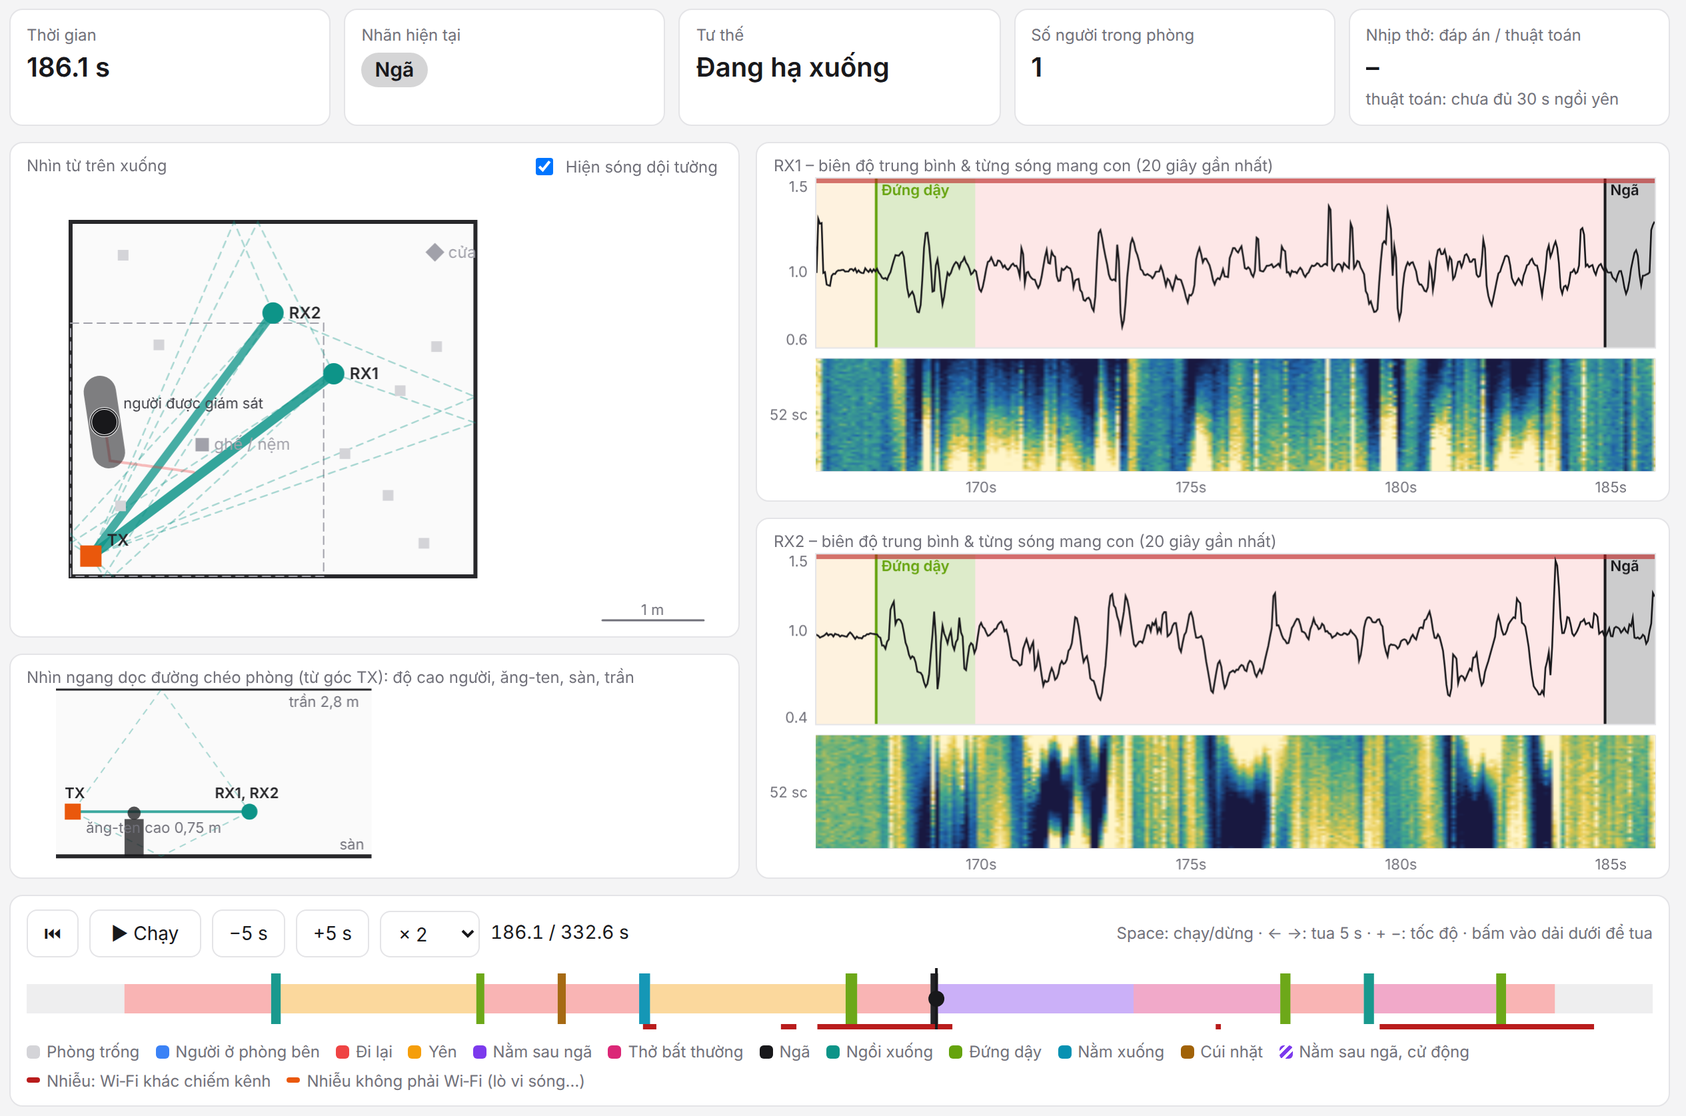
\includegraphics[width=\linewidth]{hinh/mo_phong_ui.png}
    \column{0.29\textwidth}
      \footnotesize
      \daumuc{Đang xem: lúc vừa ngã}
      \begin{itemize}
        \item \textbf{Phòng nhìn từ trên:} người, đường sóng TX → RX1, RX2 đậm lên khi bị che.
        \item \textbf{Nhìn ngang:} độ cao người, ăng‑ten, sàn, trần.
        \item \textbf{Biên độ CSI} và bản đồ nhiệt 52 sóng mang con của từng RX, 20 s gần nhất.
        \item \textbf{Dải thời gian:} nhãn cả buổi, đợt nhiễu kênh; tua tới từng sự kiện.
      \end{itemize}
  \end{columns}
\end{frame}

% ====================================================================== 14. Kết quả
\begin{frame}{Kết quả mô phỏng qua ba vòng tối ưu}
  \begin{columns}[T,onlytextwidth]
    \column{0.58\textwidth}
      \begin{tikzpicture}
        \begin{axis}[nhom8, name=a, width=43mm, height=40mm, ybar, bar width=6mm, ymin=0, ymax=53,
            xtick={1,2,3}, xticklabels={Vòng 1,Vòng 2,Vòng 3}, enlarge x limits=0.25,
            title={Ngã bắt được / 53}, nodes near coords]
          \addplot[fill=navy!70,draw=none] coordinates {(1,34) (2,39) (3,44)};
        \end{axis}
        \begin{axis}[nhom8, at={(a.east)}, anchor=west, xshift=12mm, width=43mm, height=40mm, ybar, bar width=6mm,
            ymin=0, ymax=16, xtick={1,2,3}, xticklabels={Vòng 1,Vòng 2,Vòng 3}, enlarge x limits=0.25,
            title={Báo ngã giả mỗi giờ}, nodes near coords]
          \addplot[fill=nhat,draw=none] coordinates {(1,14) (2,6.7) (3,5.1)};
        \end{axis}
      \end{tikzpicture}
      \vskip3mm
      {\scriptsize\color{xam}Vòng 2: gộp kết quả hai board. Vòng 3: bộ cột gọn, cờ kênh bận, cân bằng lại phần đo
        nhịp thở.\par}
      \vskip1.5mm
      {\scriptsize\color{xam}Dữ liệu mô phỏng: chỉ để kiểm tra luồng xử lý và chọn thiết kế; kết quả chính sẽ đo trên
        dữ liệu thật.\par}
    \column{0.36\textwidth}
      \vskip2.6mm
      \theso{83\,\% \normalsize(44/53)}{ngã bắt được, trễ trung bình 13,6 s; ngã rồi giãy 17/18}\par\vskip2.5mm
      \theso{0,1\,\%}{1 người bị gọi nhầm là nhiều người}\par\vskip2.5mm
      \theso{5/8}{lần bất động lâu bắt được}\par\vskip2.5mm
      \theso{6/21 · 1/12}{thở nhanh/chậm · nín thở bắt được: \textbf{điểm yếu nhất}}
  \end{columns}
\end{frame}

% ====================================================================== 15. Kết luận
\section{Kết luận và kế hoạch}\muc{5. Kết luận và kế hoạch}
\begin{frame}{Kết luận và kế hoạch}
  \begin{columns}[T,onlytextwidth]
    \column{0.5\textwidth}
      \small
      \daumuc{Đã đạt được}
      \begin{itemize}
        \item Bài toán thực tế rõ ràng; nhánh thiết bị có chỗ trong luồng cảnh báo.
        \item Pipeline đủ 4 tầng và bộ cảnh báo, đánh giá theo sự kiện trên mô phỏng.
      \end{itemize}
      \vskip3mm
      \daumuc{Hạn chế}
      \begin{itemize}
        \item Mới có dữ liệu mô phỏng; kết quả thật có thể khác nhiều.
        \item Đo nhịp thở và phát hiện nín thở còn yếu.
      \end{itemize}
    \column{0.44\textwidth}
      \small
      \daumuc{Kế hoạch}
      \vskip1.5mm
      \begin{tikzpicture}[font=\scriptsize]
        \draw[duong,line width=0.7pt] (0,0) -- (0,-36mm);
        \foreach \i/\w/\v in {0/Tuần 1/{Firmware TX và RX; thu, ghi nhãn dữ liệu thật},
                              1/Tuần 2/{Train lại trên dữ liệu thật; firmware sniffer},
                              2/Tuần 3/{Mô hình 6 s, nhịp thở trên board; Telegram, trang web},
                              3/Tuần 4/{Demo thời gian thực; đánh giá; báo cáo cuối kỳ}} {
          \fill[white] (0,-\i*12mm) circle (1.3mm);
          \draw[navy,line width=0.7pt] (0,-\i*12mm) circle (1.1mm);
          \node[anchor=west,font=\scriptsize\bfseries,text=navy,inner sep=0pt] at (3.5mm,-\i*12mm) {\w};
          \node[anchor=north west,text width=52mm,align=flush left,font=\scriptsize,inner sep=0pt] at (3.5mm,-\i*12mm-2.4mm) {\v};}
      \end{tikzpicture}
  \end{columns}
\end{frame}

% ====================================================================== 16. Cảm ơn
\begin{frame}
  \vfill
  \centering
  {\fontsize{22pt}{28pt}\selectfont\bfseries\color{navy}Cảm ơn thầy và các bạn\\đã lắng nghe\par}
  \vskip4mm
  {\color{navy}\rule{14mm}{0.8pt}}\par
  \vfill
\end{frame}

\end{document}